%\section{Une section}

% remarque : pour qu'un mot se retrouve dans le lexique : \MotDefinition{asymptote horizontale}{} 

\begin{methode*1}[Construire le symétrique d'un point à l'équerre]

\begin{aconnaitre}
Le \MotDefinition{symétrique d'un point $P$}{} par rapport à une droite $d$ est le point $S$ tel que la droite $d$ soit la médiatrice du segment $[PS]$. 
\end{aconnaitre}

\begin{exemple*1}
Construis le point $S$, symétrique de $P$ par rapport à la droite $d$, en utilisant l'équerre : \\[0.5em]
\begin{tabularx}{\textwidth}{X|X|X}
 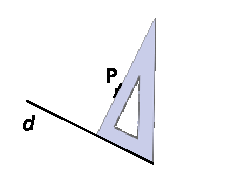
\includegraphics[width=2.4cm]{equerredP} &  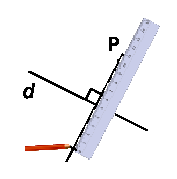
\includegraphics[width=2.4cm]{equerredP_perp} & \includegraphics[width=2.2cm]{symP} \\ 
 On construit la droite perpendiculaire à la droite $d$ passant par le point $P$. & On reporte la distance de $P$ à $(d)$ de l'autre côté de $d$ sur cette perpendiculaire. & On obtient ainsi le point $S$ tel que $d$ soit la médiatrice de $[PS]$.\\
\end{tabularx} \\
 \end{exemple*1}


\exercice
Trace deux droites sécantes $d'$ et $d''$ puis place un point $A$ qui n'appartient ni à $d'$, ni à $d''$. Construis les symétriques $A'$ et $A''$ de $A$ par rapport à $d'$ et à $d''$.
%\correction
 
\end{methode*1}

%%%%%%%%%%%%%%%%%%%%%%%%%%%%%%%%%%%%%%%%%%%%%%%%%%%%%%%%%%%%%%%%%%%%%

\begin{methode*1}[Construire le symétrique d'un point au compas]

\begin{aconnaitre}
Si $A$ et $B$ sont symétriques par rapport à une droite $d$ alors chaque point de la droite $d$ est \MotDefinition{équidistant}{} de $A$ et de $B$. 
\end{aconnaitre}

\begin{exemple*1}
Construis le point $S$, symétrique de $P$ par rapport à la droite $d$, au compas seul : \\[0.5em]
\begin{tabularx}{\textwidth}{X|X|X}
 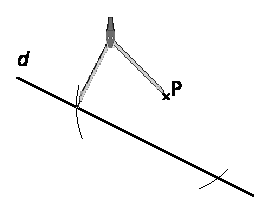
\includegraphics[width=3cm]{compasdP} &  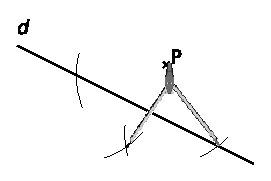
\includegraphics[width=3cm]{compasdP2} & 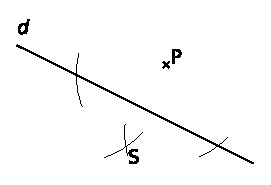
\includegraphics[width=3cm]{pointsdPS} \\ 
 On trace un arc de cercle de centre $P$ qui coupe l'axe en deux points. & De l'autre côté de la droite $d$, on trace deux arcs de cercle de même rayon et de centre les deux points précédents. & Ces deux arcs se coupent en un point qui est le point $S$, symétrique de $P$ par rapport à $d$. \\
\end{tabularx} \\
 \end{exemple*1}


\exercice
Construis un triangle $ABC$. Construis le point $D$, symétrique de $B$ par rapport à $(AC)$.
%\correction
 
\end{methode*1}

%%%%%%%%%%%%%%%%%%%%%%%%%%%%%%%%%%%%%%%%%%%%%%%%%%%%%%%%%%%%%%%%%%%%%

\begin{methode*1}[Utiliser les propriétés de la symétrie axiale]

\begin{aconnaitre}
La symétrie axiale conserve les \textbf{longueurs, l'alignement, les angles et les aires}.
\end{aconnaitre}

\begin{exemple*1}
Soit un triangle $ABC$ rectangle en $B$ tel que $AB = 3,3$ cm et $BC = 6$ cm. Quelle est la nature du triangle $A'B'C'$ symétrique de $ABC$ par rapport à la droite $(AC)$ ? Justifie. \\[0.5em]
\begin{minipage}[c]{0.4\linewidth}
 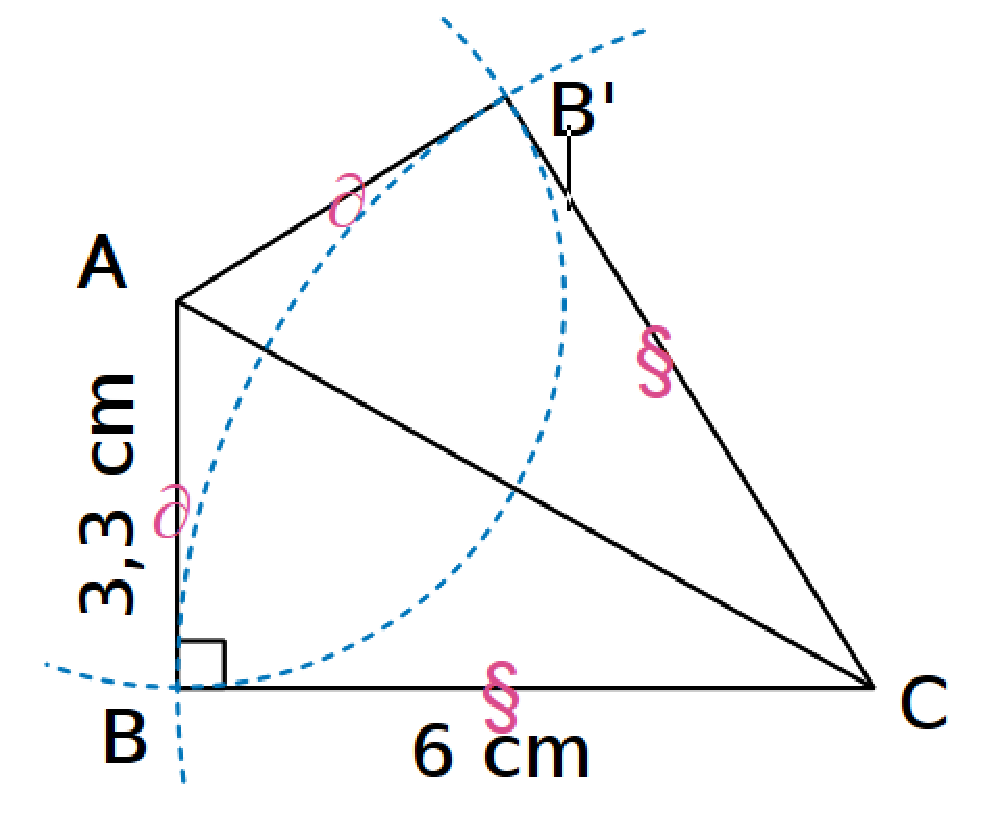
\includegraphics[width=4.3cm]{symABBC} \qquad
 \end{minipage}
 \begin{minipage}[c]{0.56\linewidth}
 \begin{itemize}
  \item $A$ et $C$ appartiennent à l'axe de symétrie, ils sont donc chacun leur propre symétrique. On appelle $B'$ le symétrique de $B$ par rapport à $(AC)$.
  \item $ABC$ est rectangle en $B$ donc $\widehat{ABC} = 90^{\circ}$. Or la symétrie axiale conserve la mesure des angles donc $\widehat{A'B'C'} = 90^{\circ}$. $A'B'C'$ est un triangle rectangle en $B'$.
  \item La symétrie axiale conserve les longueurs donc $AB = AB' = 3,3$ cm et $CB = CB' = 6$ cm.
  \end{itemize}
 \end{minipage} \\
 \end{exemple*1}


\exercice
Trace une droite $d$ et un point $F$ qui n'est pas sur $d$. Trace le cercle de centre $F$ et de rayon 5 cm. Trace son symétrique par rapport à $d$.
%\correction
 
\end{methode*1}

%%%%%%%%%%%%%%%%%%%%%%%%%%%%%%%%%%%%%%%%%%%%%%%%%%%%%%%%%%%%%%%%%%%%%

\begin{methode*1}[Construire le symétrique d'un point]

\begin{aconnaitre}
\MotDefinition{Deux points $A$ et $A'$ sont symétriques par rapport à $O$}{} lorsque $O$ est le milieu du segment $[AA']$. 
\end{aconnaitre}

\begin{exemple*1}
Trace le point $A'$ tel que les points $A$ et $A'$ soient symétriques par rapport à $O$ : \\[0.5em]
\begin{tabularx}{\textwidth}{X|X|X}
 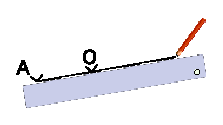
\includegraphics[width=3cm]{regleAO} &  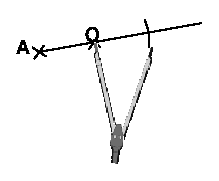
\includegraphics[width=3cm]{compasAO} & 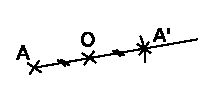
\includegraphics[width=3cm]{pointsAOA} \\ 
 On trace la demi-droite $[AO)$. & On trace un arc de cercle de centre $O$ et de rayon $OA$. Il coupe la demi-droite $[AO)$ en un point. & On place le point $A'$ à l'intersection de la demi-droite $[AO)$ et de l'arc de cercle. On code la figure. \\
\end{tabularx} \\
 \end{exemple*1}


\exercice
Trace un segment $[AB]$ de 5 cm de longueur puis construis le point $C$ symétrique de $B$ par rapport à $A$.
%\correction

\exercice
Trace un segment $[RT]$ de 8,4 cm de longueur, puis place le point $W$ tel que $R$ et $T$ soient symétriques par rapport au point $W$.
%\correction
 
\end{methode*1}

%%%%%%%%%%%%%%%%%%%%%%%%%%%%%%%%%%%%%%%%%%%%%%%%%%%%%%%%%%%%%%%%%%%%%

\begin{methode*1}[Construire le symétrique d'une figure]

\begin{aconnaitre}
\MotDefinition{Deux figures symétriques par rapport à un point}{} sont superposables après un demi-tour autour de ce point. 
\end{aconnaitre}

\begin{exemple*1}
Construis le symétrique de la figure $ABCD$ par rapport au point $O$ : \\[0.5em]
\begin{tabularx}{\textwidth}{X|X|X}
 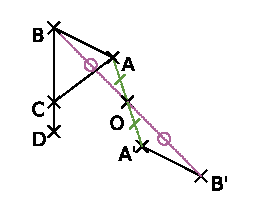
\includegraphics[width=3cm]{figure_sym1} &  \includegraphics[width=3cm]{figure_sym2} & 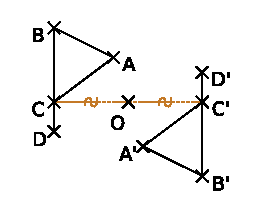
\includegraphics[width=3cm]{figure_sym3} \\ 
 On construit les points $A'$ et $B'$, symétriques des points $A$ et $B$ par rapport à $O$. On trace le segment $[A'B']$. & On construit  le point $D'$, symétrique du point $D$ par rapport à $O$. On trace le segment $[B'D']$. & On construit le point $C'$, symétrique du point $C$ par rapport à $O$. On trace le segment $[A'C']$. \\
\end{tabularx} \\
 \end{exemple*1}


\exercice
Trace un rectangle $ABCD$ tel que $AB = 4$ cm et $BC = 2,5$ cm. Trace le cercle de centre $B$ passant par $C$. Construis le symétrique de cette figure par rapport au point $D$.
%\correction
 
\end{methode*1}

%%%%%%%%%%%%%%%%%%%%%%%%%%%%%%%%%%%%%%%%%%%%%%%%%%%%%%%%%%%%%%%%%%%%%

\begin{methode*1}[Utiliser les propriétés de la symétrie centrale]

\begin{aconnaitre}
Si deux segments sont symétriques par rapport à un point alors \textbf{ils ont la même longueur}.

Si deux angles sont symétriques par rapport à un point alors \textbf{ils ont la même mesure}.

La symétrie centrale \textbf{conserve le périmètre et l'aire}.
\end{aconnaitre}

\begin{exemple*1}
Un triangle $PIC$ a un périmètre de 16,4 cm. Quel est le périmètre du triangle $PI'C'$ image de $PIC$ par la symétrie de centre $P$ ? Justifie ta réponse.\\[1em]
\correction
Les triangles $PIC$ et $PI'C'$ sont symétriques par rapport à un point : ils ont donc le même périmètre, c'est à dire 16,4 cm.
 \end{exemple*1}


\exercice
Les angles $\widehat{xOy}$ et $\widehat{x'Oy'}$, dont les mesures respectives sont $54^{\circ}$ et $55^{\circ}$, sont-ils symétriques par rapport au point $O$ ? Justifie ta réponse.
%\correction

\exercice
$ESV$ est un triangle rectangle en $E$. Quelle est la nature du triangle $E'S'V'$ image de $ESV$ par une symétrie centrale ? Justifie ta réponse.
%\correction
 
\end{methode*1}

